\section{Related work}
%
\myparagraph{Few-shot learning}
%
Research literature on few-shot learning exhibits great diversity. 
%
In this section, we focus on methods using the supervised meta-learning paradigm~\cite{Hinton1987, Thrun1998, FinnAL17} most relevant to ours
%
and compared to in the experiments. 
%
We can divide these methods into three categories.
1)~\emph{Metric learning} methods \cite{VinyalsBLKW16, SnellSZ17, SungCVPR2018} learn a similarity space in which learning is efficient for few-shot examples.
%
2)~\emph{Memory network} methods \cite{MunkhdalaiICML2017, SantoroBBWL16, OreshkinNIPS18, MishraICLR2018} learn to store ``experience'' when learning seen tasks and then generalize that to unseen tasks.
%
3)~\emph{Gradient descent} based methods \cite{FinnAL17, RaviICLR2017, LeeICML18, GrantICLR2018, ZhangNIPS2018MetaGAN} have a specific \emph{meta-learner} that learns to adapt a specific \emph{base-learner} (to few-shot examples) through different tasks. E.g. MAML \cite{FinnAL17} uses a meta-learner that learns to effectively initialize a base-learner for a new learning task.
%
Meta-learner optimization is done by gradient descent using the validation loss of the base-learner.
%
Our method is closely related.
%
An important difference is that our MTL approach leverages transfer learning and benefits from referencing neuron knowledge in pre-trained deep nets. Although MAML can start from a pre-trained network, its element-wise fine-tuning makes it hard to learn deep nets without overfitting (validated in our experiments).
%

\begin{figure*}[htp]
  \centering
  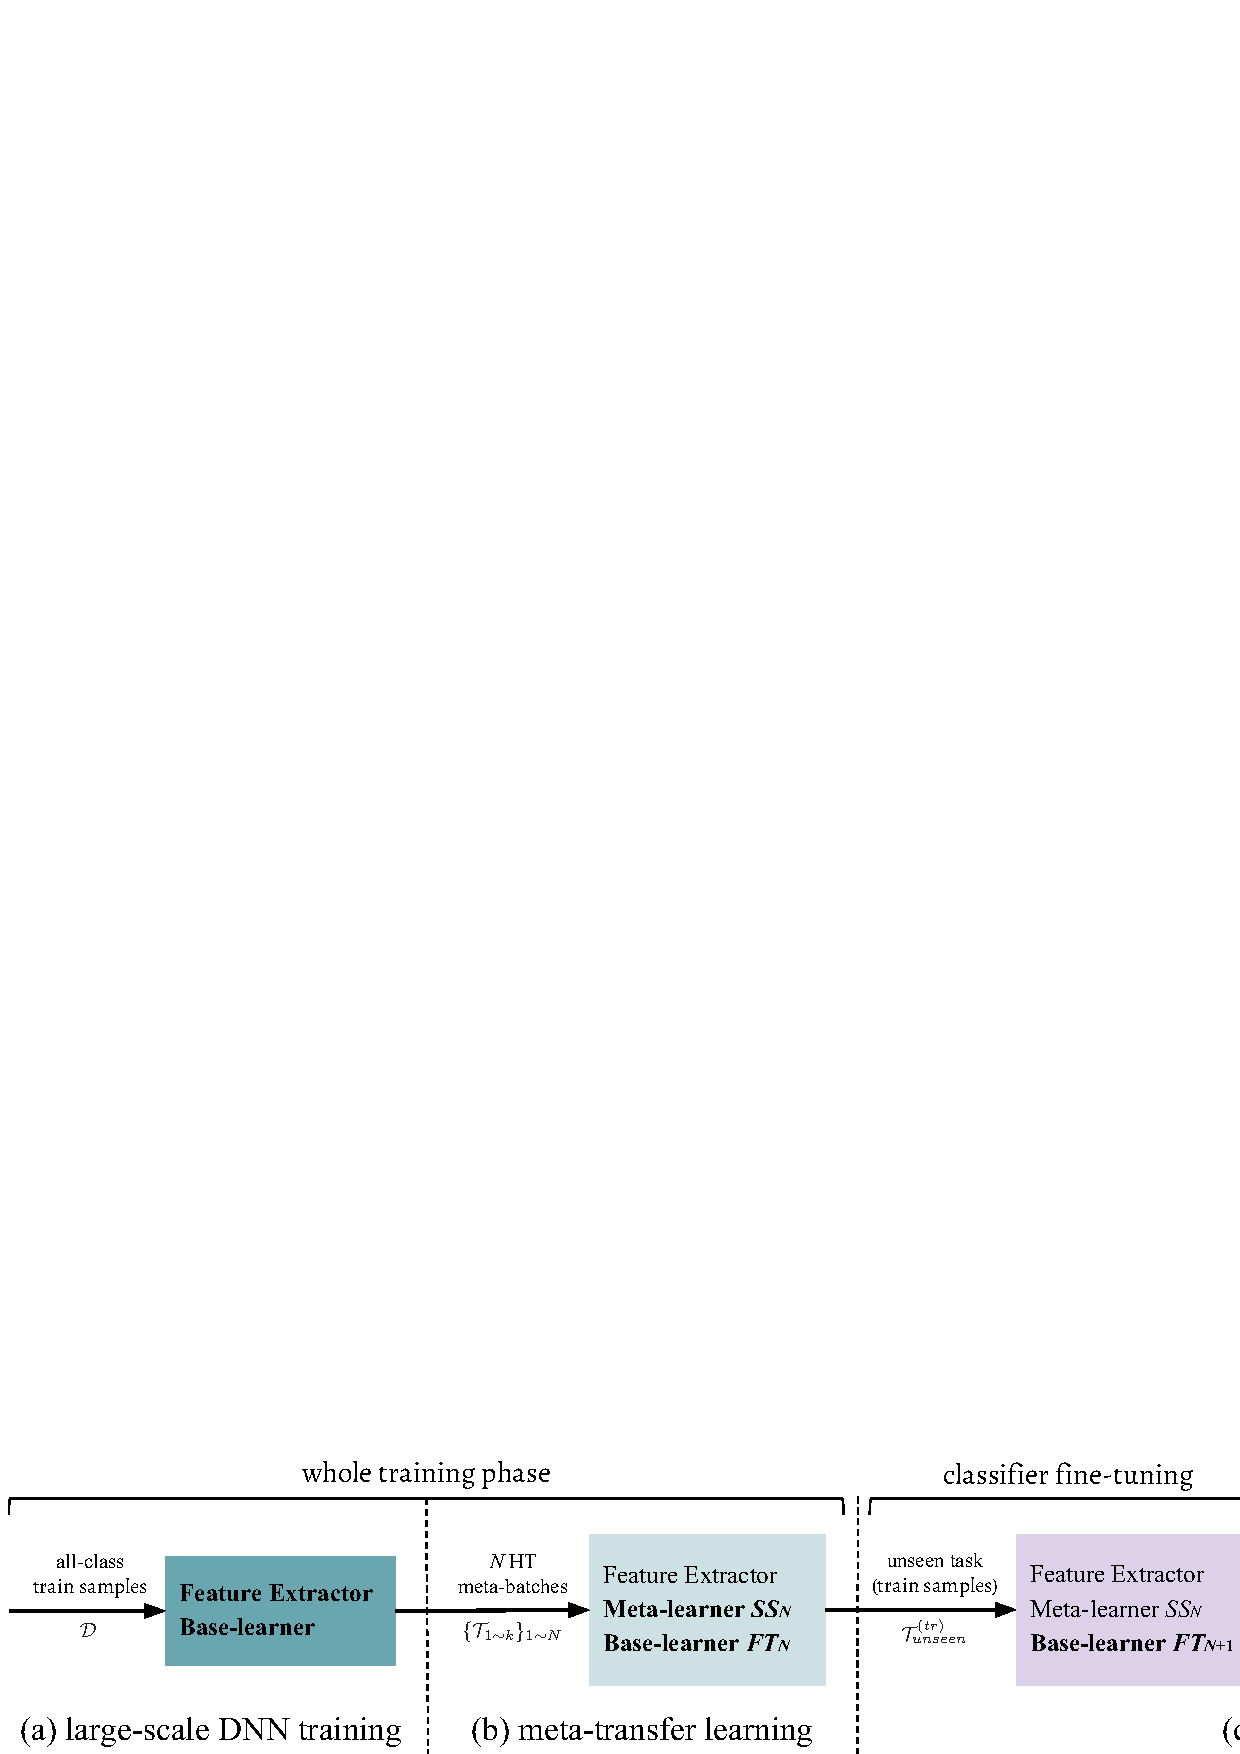
\includegraphics[width=0.99\linewidth]{figures/main_framework_meta_transf_hard_task.pdf}
     \caption{The pipeline of our proposed few-shot learning method, including three phases: (a) DNN training on large-scale data, i.e. using all training datapoints (Section~\ref{sec_large_scale_pretrain}); (b) Meta-transfer learning (MTL) that learns the parameters of \emph{Scaling} and \emph{Shifting} (\emph{SS}), based on the pre-trained feature extractor (Section~\ref{sec_meta_transfer}). Learning is scheduled by the proposed HT meta-batch (Section~\ref{sec_HT}); and (c) meta-test is done for an unseen task which consists of a base-learner (classifier) \emph{Fine-Tuning} (\emph{FT}) stage and a final evaluation stage, described in the last paragraph in Section~\ref{sec_preli}. 
     Input data are along with arrows. Modules with names in bold get updated at corresponding phases. Specifically, \emph{SS} parameters are learned by meta-training but fixed during meta-test. Base-learner parameters are optimized for every task.}
     \vspace{-0.3cm}
  \label{main_framework_meta_transf_hard_task}
\end{figure*}


\myparagraph{Transfer learning}
\emph{What} and \emph{how} to transfer are key issues to be addressed in transfer learning, as different methods are applied to different source-target domains and bridge different transfer knowledge~\cite{PanTKY11, YangICDM07, WeiICML2018, AmirCVPR18}.
%
For deep models, a powerful transfer method is adapting a pre-trained model for a new task, often called \emph{fine-tuning} (\emph{FT}). Models pre-trained on large-scale datasets have proven to generalize better than randomly initialized ones \cite{Erhan10}.
%
Another popular transfer method is taking pre-trained networks as backbone and adding high-level functions, e.g. for object detection and recognition~\cite{HuangCVPR017, Sun_2017_CVPR, Sun_2018_CVPR} and image segmentation~\cite{He_MaskRCNN17,ChenPAMI18}.
%
Our meta-transfer learning leverages the idea of transferring
pre-trained weights and aims to meta-learn how to effectively transfer. 
%
In this paper, large-scale trained DNN weights are \emph{what} to transfer, and the operations of \emph{Scaling} and \emph{Shifting} indicate \emph{how} to transfer.
Similar operations have been used to modulating the per-feature-map distribution of activations for visual reasoning~\cite{FiLM2018}.

Some few-shot learning methods have been proposed to use pre-trained weights as initialization \cite{Keshari18, MishraICLR2018, QiaoCVPR2018, ScottNIPS2018, Rusu2019}. Typically, weights are fine-tuned for each task, while we learn a meta-transfer learner through all tasks, which is different in terms of the underlying learning paradigm. 
%

\myparagraph{Curriculum learning \& Hard sample mining}
Curriculum learning was proposed by Bengio \emph{et al}. \cite{BengioLCW09} and is popular for multi-task learning~\cite{PentinaCVPR15, SarafianosGNK17, WeinshallCA18, GravesICML2017}.
They showed that instead of observing samples at random it is better to organize samples in a meaningful way so that fast convergence, effective learning and better generalization can be achieved.
Pentina \emph{et al}. \cite{PentinaCVPR15} use adaptive SVM classifiers to evaluate task difficulty for later organization. Differently, our MTL method does task evaluation online at the phase of episode test, without needing any auxiliary model.

Hard sample mining was proposed by Shrivastava \emph{et al}.~\cite{ShrivastavaGG16} for object detection. It treats image proposals overlapped with ground truth as hard negative samples. Training on more confusing data enables the model to achieve higher robustness and better performance~\cite{CanevetF16, HarwoodGCRD17, DalalT05}. 
Inspired by this, we sample harder tasks online and make our MTL learner ``grow faster and stronger through more hardness''. In our experiments, we show that this can be generalized to enhance other meta-learning methods, e.g. MAML~\cite{FinnAL17}.
%
%

\section{Preliminary}
\label{sec_preli}

We introduce the problem setup and notations of meta-learning, following related work~\cite{VinyalsBLKW16, RaviICLR2017, FinnAL17, OreshkinNIPS18}.

\myparagraph{Meta-learning} consists of two phases: meta-train and meta-test. A meta-training example is a classification task $\mathcal{T}$ sampled from a distribution $p(\mathcal{T})$. 
%
$\mathcal{T}$ is called episode, including a training split $\mathcal{T}^{(tr)}$ to optimize the base-learner, and a test split $\mathcal{T}^{(te)}$ to optimize the meta-learner. 
%
In particular, meta-training aims to learn from a number of episodes $\{\mathcal{T}\}$ sampled from $p(\mathcal{T})$.
%
%
An unseen task $\mathcal{T}_{unseen}$ in meta-test will start from that experience of the meta-learner and adapt the base-learner. The final evaluation is done by testing a set of unseen datapoints $\mathcal{T}^{(te)}_{unseen}$.
%


\myparagraph{Meta-training phase.} 
%
This phase aims to learn a meta-learner from multiple episodes.
In each episode, meta-training has a two-stage optimization. 
%
Stage-1 is called base-learning, where the cross-entropy loss is used to optimize the parameters of the base-learner.
%
Stage-2 contains a feed-forward test on episode test datapoints. The test loss is used to optimize the parameters of the meta-learner.
%
Specifically, given an episode $\mathcal{T} \in p(\mathcal{T})$, the base-learner $\theta_\mathcal{T}$ is learned from episode training data $\mathcal{T}^{(tr)}$ and its corresponding loss $\mathcal{L}_{\mathcal{T}}(\theta_\mathcal{T}, \mathcal{T}^{(tr)})$. 
%
After optimizing this loss, the base-learner has parameters $\tilde{\theta}_\mathcal{T}$. 
%
Then, the meta-learner is updated using test loss $\mathcal{L}_{\mathcal{T}}(\tilde{\theta}_\mathcal{T}, \mathcal{T}^{(te)})$. 
%
After meta-training on all episodes, the meta-learner is optimized by test losses $\{\mathcal{L}_{\mathcal{T}}(\tilde{\theta}_\mathcal{T}, \mathcal{T}^{(te)})\}_{\mathcal{T} \in p(\mathcal{T})}$. Therefore, the number of meta-learner updates equals to the number of episodes.

\myparagraph{Meta-test phase.} 
This phase aims to test the performance of the trained meta-learner for fast adaptation to unseen task.
Given $\mathcal{T}_{unseen}$, the meta-learner $\tilde{\theta}_\mathcal{T}$ teaches the base-learner $\theta_{\mathcal{T}_{unseen}}$ to adapt to the objective of $\mathcal{T}_{unseen}$ by some means, e.g. through initialization~\cite{FinnAL17}. 
%
Then, the test result on $\mathcal{T}^{(te)}_{unseen}$ is used to evaluate the meta-learning approach. 
%
If there are multiple unseen tasks $\{\mathcal{T}_{unseen}\}$, the average result on $\{\mathcal{T}^{(te)}_{unseen}\}$ will be the final evaluation.
